\documentclass[draft]{article}

\usepackage{tikz}
\usepackage{amsmath, amssymb, mathtools, amsthm}
\usepackage{enumitem}
\usepackage{theoremref}
\usepackage[english]{babel}
\usepackage{microtype}

\usepackage[margin=1.5in]{geometry}

\usepackage[backend=bibtex, style=numeric, sorting=anyt,
url=false, sortcites=true]{biblatex}
\addbibresource{thebib.bib}

\usetikzlibrary{arrows, calc, patterns, positioning, shapes}
\usetikzlibrary{decorations.pathmorphing, backgrounds, scopes}


\DeclarePairedDelimiter\abs{\lvert}{\rvert}
\newcommand{\sqf}[2]{#1_1 #1_2 \mathellipsis #1_{#2}}
\newcommand{\qs}{\sqf{q}{s}}
\newcommand{\ps}{\sqf{p}{s}}
\newcommand{\rs}{\sqf{r}{s}}
\newcommand{\ufd}{p_1^{\alpha_1} p_2^{\alpha_2} \cdots p_s^{\alpha_s}}
\newcommand{\ufdsh}{p_1^{\alpha_1} \cdots p_s^{\alpha_s}}
\newcommand{\fbr}[1]{g^{-1}{(#1)}}
\newcommand{\aut}[1]{\operatorname{Aut}(#1)}
\newcommand{\cyc}[1]{\operatorname{C}_{#1}}
\newcommand{\gl}[2]{\operatorname{GL}(#1, \mathbb{F}_#2)}
\newcommand{\Mod}[1]{\ (\mathrm{mod} \ #1)}
\newcommand{\qo}{\tilde{q}}
\newcommand{\pin}{\tilde{p}}
\newcommand{\tilpi}{\tilde{\pi}}
\newcommand{\piga}{\pi_\Gamma}
\newcommand{\pila}{\pi_\Lambda}
\newcommand{\fibo}[1]{F_{#1}}
\newcommand{\qlame}{\Lambda_{5,\text{I}}}
\newcommand{\qlamz}{\Lambda_{5,\text{II}}}
\newcommand{\qlamd}{\Lambda_{5,\text{III}}}
\newcommand{\m}[1]{\text{M}_{#1}}

\NewDocumentCommand{\listspace}{}{\linespread{0.9}\selectfont}
\NewDocumentCommand{\textspace}{}{\linespread{1}\selectfont}
\NewDocumentCommand{\eqnspace}{}{\vspace{-0.5\baselineskip}}
\NewDocumentCommand{\case}{m}{\sffamily \textbf{Case #1.} \rmfamily }
\NewDocumentCommand{\hold}{m}{Hölder}
\NewDocumentCommand{\hg}{m}{Hölder graph}
\NewDocumentCommand{\hgs}{m}{Hölder graphs}


\theoremstyle{plain}
\newtheorem{thm}{Theorem}[section]
\newtheorem{fact}{Theorem}[section]
\newtheorem{lem}{Lemma}[section]
\newtheorem{prop}{Proposition}[section]
\newtheorem*{quest}{Question}
\newtheorem{cor}[prop]{Corollary}
\newtheorem*{conj}{Conjecture}

\theoremstyle{definition}
\newtheorem*{defn}{Definition}

\setenumerate[1]{label=\alph*.}
\setenumerate[2]{label=\alph*.}
%\setlist{noitemsep, nolistsep}

\tikzset
{%
point/.style={fill=black, draw, circle, inner sep=0.042cm, outer sep=0.12cm},
soint/.style={fill=black, draw, circle, inner sep=0.022cm, outer sep=0.1cm},
lambda/.pic={
	\node [point,label=below:{#1}] (bx) {};
	\node [point,label=right:{$\alpha$},right=of bx, yshift=7.3mm] (x) {};
	\node [point,label=right:{$\beta$}, right=of bx, yshift=-7.3mm] (y) {};
	\path [->] (bx) edge[color=red, dashed] (x)
	(bx) edge (y);
},
walk/.pic={
	\node [soint] (a) {};
	\node [soint,right=of a] (b) {};
	\path [->] (a) edge (b);
},
twalk/.pic={
	\node [soint] (a) {};
	\node [soint,right=of a] (b) {};
	\node [soint, right=of b] (c) {};
	\path [->] (a) edge (b)
	(b) edge (c);
},
ewalk/.pic={
	\node [soint] (a) {};
	\node [soint, right=of a] (b) {};
},
w/.style={baseline=-0.4ex},
ww/.style={baseline=-0.4ex, node distance=0.37cm}
}

% tasks:
% improve \hold{1} /
% work on the introduction
% do Lucas, do more /
% fix spacing issues [after citations]
% finishing \hold{1} case work in lambda(n) = 4 [requires TikZ]
% write summary of the results
% do the citations
% do the graphs [requires TikZ]
% finish the first proofreading

\begin{document}
\title{On the group-counting function}
\author{Aban}
\maketitle

\begin{abstract}
	Let $g(n)$ denote the number of groups of order $n$ up to isomorphism. We solve the equations $g(n) = 6$ and $g(n) = 7$.
\end{abstract}

\section{Introduction}
The function $g(n)$, counting isomorphism types of groups of order $n$, has various interesting arithmetical properties. It is not hard to see that $g(p) = 1$ for all primes $p$. However, primes are not the only such numbers: We have $g(15) = 1$, and in fact, $g(pq) = 1$ whenever $p, q$ are primes with $q \equiv 1 \Mod{p}$. This raises the question: Which $n$ satisfy $g(n) = 1$? As $\cyc{n} = \mathbb{Z}/n\mathbb{Z}$, this is equivalent to finding $n$ such that all groups of order $n$ are cyclic.

This can be generalized in two different directions. On the one hand, we can take a group theoretic property $\mathcal{P}$ and attempt to characterize all $P$-\emph{numbers}, that is, all $n$ such that every group of order $n$ has property $\mathcal{P}$. This question is old: Dickson {\cite{dickson}} has characterized abelian numbers over a century ago. Nilpotent numbers {\cite{pazderski}} and cyclic numbers {\cite{szele}} have also been characterized (for a modern treatment, see {\cite{nilnumb}}). In {\cite{mueller}}, this problem is solved for $\mathcal{P} = $ nilpotent of class at most $c$, which generalizes the last three problems.

On the other hand, we can simply consider $g(n) = k$ for a fixed $k$. Miller answers this question for $k = 1, 2, 3$ in {\cite{miller1}} and for $k = 4, 5$ in {\cite{miller2}}, but the result has been re-derived multiple times: For instance, the case $k = 3$ is handled in {\cite{olsson}} and $1 \le k \le 4$ in {\cite{gnumoas}}. It is an open problem whether we every number is $g(n)$ for some $n$, but there is strong evidence that this is the case even when one restricts to odd, squarefree $n$. The two directions are not too separate: It turns out, for example, that $g(n)$ is a power of $2$ whenever $n$ is an abelian number.

A beautiful formula for $g(n)$ when $n$ is squarefree has been discovered by \hold{1} {\cite[Theorem~5.1]{gnumoas}}. An instance of it is that, if $p, q, r$ are primes and $q \equiv r \equiv 1 \Mod{p}$, for example, then $g(pqr) = p + 2$, already showing that the image of $g$ is infinite. There is no similarly explicit formula for all cubefree $n$, but there is an efficient algorithm for enumerating all groups of cubefree order {\cite{cubefree}}, and there are relatively simple formulae for $g(n)$ when $n$ has a few number of prime factors.

Using the Krull-Schmidt theorem {\cite{hungerford}}, one can see that $g(ab) \ge g(a)g(b)$. Since $g(p^2) = 2, g(p^3) = 5$ and $g(p^4) \ge 14$ for all primes $p$ {see, e.g., \cite[Theorem~3.1]{gnumoas}}, we see that we only consider fourth-power-free values for $n$. In fact, we will see that $g(n) = 6, 7$ for non-cubefree $n$ is relatively rare, so we will mostly be working with cubefree $n$. We will use directed graphs heavily to simplify the arguments: The vertices will be the prime powers dividing $n$, and the edges essentially indicate that nontrivial semidirect products exist.

\section{\hgs{1}}
\subsection{\hold{1}'s formula}
For a squarefree $n$, a prime factor $p$ and a subset $\pi$ of its set of prime factors $\Gamma$, we let $v(p, \pi)$ denote the number of primes $\pi$ that $p$ is related to, that is, the number of primes $q$ in $\pi$ such that $q \equiv 1 \Mod{p}$. Then we have
\begin{fact}[\textbf{\hold{1}'s formula}]\thlabel{euholder} In this notation, we have
	\begin{equation*}
		g(n) = \sum_{\sigma \subseteq \Gamma} \prod_{p \notin \sigma} \frac{p^{v(p, \sigma)} - 1}{p - 1}
	\end{equation*}
\end{fact}
\begin{proof} See {\cite[Theorem~5.1]{gnumoas}}. \end{proof}

It is therefore natural to define the \emph{\hg{1}} of a squarefree integer $n$ to be unlabeled directed graph whose vertices are the prime factors, and where we draw an edge $p \rightarrow q$ precisely when $p$ is related to $q$. Observe also that when the out-degree of every vertex is at most 1, it follows that $g(n)$ depends solely on the \hg{1}, and therefore we are justified in speaking of $g(\Gamma).$ We call both $n$ and $\Gamma$ \emph{regular} in this case. We will occasionally treat directed acyclic graphs $\Gamma$ with only the vertices whose out-degree exceeds 1 labeled. In this case, we can still speak of $g(\Gamma)$ without ambiguity, as it will be independent from the labels of the rest of the vertices. Observe also that a given (unlabeled) directed acyclic graph is always realizable as the \hg{1} of some odd squarefree integer, via Dirichlet's theorem on arithmetic progressions.

We generalize this to arbitrary $n$ as follows. The vertices are now the prime powers, and an edge $p^\alpha \rightarrow q^\beta$ exists precisely when $q^j \equiv 1 \Mod{p^i}$ for some $1 \le i \le \alpha$ and $1 \le j \le \beta$. The edge will be labeled $(i, j)$ where $j$ is the smallest such integer, and $i$ the largest, and we drop $i$ if $\alpha = 1$ and similarly for $j$. We call this the \emph{generalized \hg{1}} for $n.$ These are not necessarily acyclic, and the labels will not be of much interest to us. In analyzing the solutions to $g(n) = k$, we will make use of this concept. To simplify notation further, we write $p^2 \dashrightarrow q$ to mean $p \parallel q - 1$. On the other hand, we write $q \dashrightarrow p^2$ to mean $q \mid p + 1$ but $q \nmid p - 1$ (that is, $p$ has order $2$ modulo $q$). We call these ``weak arrows.``

%\emph{Remark.} From Dirichlet's theorem on arithmetic progression see that every directed acyclic graph is the \hg{1} of infinitely many squarefree integers: Ultimately, choosing the next prime in the factorization amounts to finding a prime satisfying some linear congruences modulo primes, and this is always possible.
In the following, we let $S(\pi, \Gamma)$ denote the summand corresponding to the subset $\pi$ in a \hg{1} $\Gamma,$ and each factor of it will be denoted $h_\Gamma(p, \pi).$ Moreover, we will call vertices $q$ with no edge $q \rightarrow v$ terminal, and vertices $p$ with no edge $v \rightarrow p$ as initial. A vertex with out-degree of at most 1 will be called regular.

If there is a vertex $p$ not connected to any vertex in $\pi,$ the entire summand $S(\pi; \Gamma)$ vanishes. Motivated by this observation, we call a subset $\pi$ \emph{central} if, for every vertex outside of it, there exists at least one edge to a vertex inside it - equivalently, if $S(\pi; \Gamma)$ does not vanish, and we let $c(\Gamma)$ denote the number of central subsets. In this notation, $g(\Gamma) \ge c(\Gamma)$ and equality holds precisely when $\Gamma$ is regular.

\subsection{Connectivity and multiplicativity}
We have already observed that $g(ab) \ge g(a)g(b).$ When does equality hold? If it does hold, then every group of order $ab$ splits as a direct product of groups of orders $a$ and $b.$ So the first condition is coprimality: If $p$ divides both $a$ and $b,$ we simply observe that the group $\cyc{a/p} \times \cyc{p^2} \times \cyc{b/p}$ does not split in this way. Next, it must be impossible to form semidirect products. If $p$ divides $b$ and $q^n$ divides $a$, we observe that $\abs{\aut{\cyc{q}^n}}$ has $q^i - 1$ as a factor for all $1 \le i \le n$, and therefore a nontrivial semidirect product exists if there is a relation $p \rightarrow q^n.$ It is therefore necessary that the generalized \hg{1} of $n = ab$ is the disjoint union of $a$ and $b$. In fact, the converse holds:

\begin{thm}\thlabel{eufrobenius}
	Suppose we have $n = ab$.
	\begin{enumerate}\listspace
		\item $g(n) = g(a)g(b).$
		\item Every group of order $n$ decomposes as a direct product of a group of order $a$ and a group of order $b.$
		\item $a$ and $b$ are coprime and arithmetically independent - that is, the generalized \hg{1} of $n$ decomposes into two disjoint subgraphs corresponding to $a$ and $b.$
	\end{enumerate} \textspace
\end{thm}
\begin{proof}
	See {\cite[Lemma~21.19]{monolith}}.
\end{proof}

\begin{prop}\thlabel{euufd}
	For positive $n,$ we have a unique factorization $n = n_1 \cdots n_k m$ where\pagebreak[3]
	\begin{enumerate} \listspace
		\item Each pair $(n_i, n_j)$ and $(n_i, m)$ is arithmetically independent.
		\item Each $n_i$ is connected with $g(n_i) \ge 2.$
		\item $m$ is cyclic, i.e., $g(m) = 1.$
	\end{enumerate} \textspace
\end{prop}
\begin{proof}
	This follows immediately from considering the generalized \hg{1} of $n$ and letting the $n_i$ be the numbers corresponding to the connected component of at least two vertices, and $m$ the product of all the labels of the isolated vertices.
\end{proof}

In solving $g(n) = k$, therefore, it makes sense to consider first the ``prime`` $n$, that is, those which do not factorize nontrivially according to the above proposition: These will be called the \emph{connected} numbers, that is, the ones with connected generalized \hg{1}. For a general $n$, we call $m$ the \emph{cyclic part} of $n$, and $n$ is \emph{cyclic-free} if $m = 1$. One application of connectivity is the following lower bound, obtained by considering non-nilpotent groups.

\begin{prop}\thlabel{eunnp}
	If $n = \ufdsh$ is connected, then $g(n) \ge g(p_1^{\alpha_1})\cdots g(p_s^{\alpha_s}) + s - 1.$
\end{prop}

\subsection{Splicing graphs}
%It is of interest to exploit the multiplicative property $g(ab) = g(a)g(b)$ in investigating the image of $g.$ In particular, we see that at least a subset of it is closed under multiplication. This shows, for example, that 7-smooth numbers(that is, numbers of the form $2^\alpha 3^\beta 5^\gamma$) are group numbers: We realize $2^\alpha$ as the image of the disjoint union of $\alpha$ graphs $\bullet \rightarrow \bullet$ and so on. If we could realize all primes as images of squarefree numbers in such a way that the preimage of any prime is infinite (or simply realized the prime powers as images of $g$ without restriction) we will have proved the surjectivity conjecture. Unfortunately,

Given graphs $\Gamma$ and $\Lambda$ with a fixed terminal vertex $\qo$ in $\Gamma$ and any vertex $\pin$ in $\Lambda$, we can make a new graph $\Gamma \rightarrow \Lambda$ by adjoining an arrow $\pin \rightarrow \qo$ to the disjoint union of $\Gamma$ and $\Lambda$. This depends on the choice of $\qo$ and $\pin$ in general, but this will be clear from context. 

\begin{prop}\thlabel{eujoin}
	In this notation, \eqnspace \begin{equation*} g(\Gamma \rightarrow \Lambda) = g(\Gamma)g(\Lambda) + g(\Gamma - \{\qo\})g(\Lambda; \pin). \end{equation*}
\end{prop}
\begin{proof}
	Let $M = \Gamma \rightarrow \Lambda.$ From a subset $\tilpi$ of $M$ we define the obvious subsets $\piga$ and $\pila.$ To simplify notation, we write $h_X(p, \pi)$ to denote the factor corresponding to $p$ in $S(\pi, X).$ We first observe that $h_M(p, \tilpi) = h_\Lambda(p, \pila)$ because no edge exists from a $\Lambda$-vertex to a $\Gamma$-vertex. Now we evaluate $S(\tilpi, M)$ for a subset $\tilpi,$ and we distinguish three cases.
	
	
	If $\qo \in \piga$, we have $h_M(p, \tilpi) = h_\Gamma(p, \piga)$ for vertex $p$ in $\Gamma$. For a vertex $p$ in $\Lambda$ the holds, because no vertex in $\Lambda$ is connected to a vertex in $\Gamma$. Thus we have $S(\tilpi, M) = S(\piga, \Gamma)S(\pila, \Lambda).$
	
	If we have $\qo\notin\piga$ and $\pin \in \pila$ we have $h_M(\qo, \tilpi) = 1$ because there is an edge $\qo \rightarrow \pin,$ and so it contributes nothing to the product. In the other front, we have $h_M(\pin, \tilpi) = h_\Lambda(\pin, \pila)$ because again no vertex in and therefore $S(\tilpi, M) = S(\piga, \Gamma - \{\qo\})S(\pila, \Lambda)$.
	
	Finally, if $\qo \notin \piga$ and $\pin\notin\pila,$ the previous analysis shows that $h_M(\qo, \tilpi) = 0$, which in turn implies that $S(\tilpi, M) = 0$ and so $\tilpi$ contributes nothing to the sum.
	
	The subsets $\tilpi$ evidently correspond bijectively to pairs $(\piga, \pila)$ with $\piga \subseteq \Gamma$ and $\pila \subseteq \Lambda.$ For the pairs with $\qo \in \piga$ we get $g(\Gamma)g(\Lambda)$. For the pairs with $\qo \notin \piga$, we need $\pin \in \pila,$ and these terms combine to give precisely $g(\Gamma - \{\qo\})g(\Lambda; \pin).$
\end{proof}

%\setenumerate{noitemsep}
\begin{cor}\thlabel{eustick} Suppose $\Gamma$ is a \hg{1} and $v$ is a disjoint vertex.\listspace
	\begin{enumerate} \listspace
		\item Fix a terminal vertex $q$ in $\Gamma$. Then $g(\Gamma \rightarrow v) = g(\Gamma) + g(\Gamma - \{q\}).$
		\item Fix an initial vertex $p$ in $\Gamma.$ Then $g(v \rightarrow \Gamma) = g(\Gamma) + g(\Gamma; p).$
	\end{enumerate}\textspace
\end{cor}

The first operation can be operated successively, that is, we can start with a graph $\Gamma_0$ with a fixed terminal vertex $q$, and define $\Gamma_{n + 1} = \Gamma_{n} \rightarrow v_{n + 1}$, where the $v_i$ are all distinct. If we let $\alpha = g(\Gamma_0 - \{q\})$ and $\beta = g(\Gamma_0)$, then the sequence $a_n = g(\Gamma_n)$ satisfies the recurrence relation $a_{n + 2} = a_{n + 1} + a_n$ with initial values $a_{-1} = \alpha$ and $a_0 = \beta$. Starting with a single vertex, we get

\begin{prop}\thlabel{eufibo}
	Let $\Phi_n$ be a directed path of $n$ vertices. Then $g(\Phi_n) = \fibo{n + 1}$, where $\fibo{n}$ is the Fibonacci sequence.
\end{prop}

An amusing consequence of this fact is this. We observe that $\Phi_{m + n} = \Phi_m \rightarrow \Phi_n$, and $g(\Phi_m - \{\text{final}\}) = \fibo{m}$ and similarly $g(\Phi_n; \text{initial}) = \fibo{n}$.
We can now apply \thref{eustick} to get the well-known identity, \eqnspace
\begin{align*}
	\fibo{m + n} &= g(\Phi_m \rightarrow Phi_{n - 1}) \\
	&= g(\Phi_m)g(\Phi_{n - 1}) + g(\Phi_m - \{\text{final}\})g(\Phi_{n - 1}; \{\text{initial}\}) \\
	&= \fibo{m + 1}\fibo{n} + \fibo{m}\fibo{n - 1}.
\end{align*}
\subsection{Some lower bounds}
We have already seen that $g(\Phi_n)$ is the Fibonacci sequence, and so it grows exponentially with $n$. By super-multiplicativity of $n$, we see that $g$ grows exponentially in the length of the longest path. We observe that it grows exponentially in the maximal in- and out-degree as .
\begin{lem}\thlabel{euinout}
	Let $r, s$ denote the in- and out-degree (respectively) of a vertex $v$ in a \hg{1} $\Gamma$ with label $p$. Then $g(\Gamma) \ge 2^r + \frac{p^s - 1}{p - 1}$.
\end{lem}
\begin{proof}
	Consider the subgraph made up by the arrows $\alpha_i \rightarrow v$ and $v \rightarrow \beta_j$ for $1 \le i \le r$ and $1 \le j \le s$. Evidently, any subset containing $v$ and the $\beta_j$ is central, and there are $2^r$ such subsets. Moreover, the complement of $\{v\}$ in this subgraph is central, and it contributes $\frac{p^s - 1}{p - 1}$. This yields the desired inequality, as adding more vertices and edges cannot decrease \nolinebreak[4] $g$.
\end{proof}
In the sequel, we will deal with generalized \hgs{1} of cube free numbers. There are only two groups of order $p^2$, namely $\cyc{p} \rtimes \cyc{p}$ and $\cyc{p}^2$. In both cases, we have an epimorphism $P \twoheadrightarrow \cyc{p}$, and thus for each semidirect product $G \rtimes \cyc{p}$, we get \textit{two} semidirect products $G \rtimes P$. On the other hand, we have a monomorphism $\aut{\cyc{p}} \hookrightarrow \aut{P}$ in both cases: For $P = \cyc{p} \rtimes \cyc{p}$ by fixing one factor and acting on the other, and for $P = \cyc{p^2}$ from the well-known fact that $\aut{P} \cong \cyc{p} \times \cyc{p - 1}$. It follows that the same observation holds for $P \rtimes G$ as well. These two facts together implies the following lemma.
\begin{lem}\thlabel{eubold}
	Let $n$ be cube-free with $s$ factors of the form $p^2$. Then $g(n) \ge 2^s g(\operatorname{rad}(n))$.
\end{lem}
\begin{proof}
	For a group $G$ of order $n_0 = \operatorname{rad}(n)$ and a prime $p \in \sigma$ where $\sigma$ is the set of prime-squared factors, we can replace the $p$-Sylow subgroup with either $\cyc{p}^2$ or $\cyc{p^2}$, since $G$ is an iterated semidirect product. This gives two choices for every prime $p$, and thus $2^s$ choices in general. It is easy to see that these are distinct groups.
\end{proof}

\section{Hunting solutions of $g(n) = 6, 7$}
In this section, we will tackle the main problem of the paper, that of finding $n$ such that $g(n) \in \{6, 7\}.$ We will call such $n$ \emph{admissible.} In the next two sections, we will consider only connected numbers $n.$ Connectivity provides an easy lower bound on $g(n).$ Here and throughout, we let $p, q, r$ be different primes. For $n = \ufd,$ we let $\lambda(n) = \sum \alpha_i$ and $\mu(n) = \max\{\alpha_i\}.$

\thref{euinout} restricts the forms of $n$ we need to consider, once one recalls $g(p^3) = 5$ and $g(p^2) = 2.$ We state this as

\begin{lem}\thlabel{euclass}
	Suppose $n$ is admissible and connected. Either $n$ is squarefree, or $n$ is a divisor of a number of one of the forms $p^2 q^2 r, p^2 q r s, p^3 qr$.
\end{lem}
\begin{proof}
	The only thing that is not obvious is the first form. \textit{A priori}, we only know that $n$ is a divisor of $p^2 q_1 \cdots q_5$. However, observe that $g(q_1 \cdots q_5) \le 7/2 = 3.5$, and thus the \hg{1} of $q_1 \cdots q_5$ has at most 3 edges. This means that at least one vertex $q_5$ is disconnected, so we can discard. Next, if we have four connected vertices, we need at least one vertex of either out- or in-degree $2$, yielding at least 4 groups, which contradicts our assumption. Thus there must be only three vertices.
\end{proof}

\subsection{Disconnected $n$}
We will deal with \textit{connected} $n$. What about disconnected $n$? This turns out to be the easiest part. Let $n = n_1 \cdots n_k m$ be the unique factorization of $n$, in the notation of \thref{euufd}, and ordered such that $g(n_i)$ is nondecreasing. The \emph{primality} of $7$ shows that, when $g(n) = 7$, we must have $k = 1$. Thus for $g(n) = 7$ it is enough to consider connected $n$. If $g(n) = 6$, either $k = 1$ of $g(n_1) = 2$ and $g(n_2) = 3$. For the sake of completeness, we re-derive the solutions here.

First, $n_1$ is cubefree and has at most one square factor. If it has none, then it must have the graph \tikz[ww] \pic {walk};. If it has one, then it cannot have any more factors. Next, we have seen that if $n_2$ is not squarefree, then it must be $p^2 q$ with $q \dashrightarrow p^2$.If it is squarefree, we cannot have a vertex with in-degree or out-degree greater than $1$ because of \thref{euinout}, so we get a path, and it must be the path of three vertices \tikz[ww] \pic {twalk};.

\subsection{Squarefree admissible numbers}
Let $i(\Gamma), o(\Gamma)$ denote the maximum in- and out-degree of a vertex in a \hg{1} $\Gamma$. If $o(\Gamma) = 3$, we get at least $1 + \frac{p^3 - 1}{p - 1} = p^2 + p + 2 \ge 8$. Thus we see that we must have $o(\Gamma) \le 2$, and for a similar reason $i(\Gamma) \le 2$. We therefore have four cases to consider.

\case{1} $i(\Gamma) = 1, o(\Gamma) = 1$. In this case $\Gamma$ is simply a path $\Phi_k$ for some $k$, and as neither 6 nor 7 is a Fibonacci number, this is never an admissible graph.

\case{2} $i(\Gamma) = 2, o(\Gamma) = 1$. It is similarly clear that is a unique vertex $v$ with in-degree 2, so let $w_1, w_2 \rightarrow v$ be arrows, and call this graph $K$. We have $g(K) = 2^2 = 4$, and the only way to add edges is by adding vertices. A new vertex $u$ can be appended via $w_1$ to get $u \rightarrow w_1$, this would give $g(K) + g(K; u) = 4 + 2 = 6$ groups via formula \thref{eustick} of \thref{eustick}, so call this new graph $Q$. We cannot extend $Q$: An arrow to $u$ will give too many groups. Adding $v \rightarrow u$ to $Q$ instead gives 5 groups using the same lemma, and we cannot extend it in any way apart form adding more vertices, which would give at least 9 groups.

\case{3} $i(\Gamma) = 1, o(\Gamma) = 2$. It is clear that there is a unique vertex with out-degree 2, so label it $p$ for some prime $p$. We get at least $p + 2$ groups, so we have $p \le 5$ and therefore $p$ is initial (there can be no other vertex labeled 2 because it will have out-degree of at least 2). We cannot add edges without adding vertices, as this would contradict $i(\Gamma) = 1$. Using \thref{eustick}, we see that adding a new vertex $s$ and an arrow $q \rightarrow s$, where $q$ is either of the two primes with an arrow from $p$, yields $p + 4$ groups. But we cannot have $p = 2$ in this case. This determines all such graphs, so we get admissible graphs when $p = 5$ in the first case and when $p = 3$ in the second case, both yielding $g = 7$.

\case{4} $i(\Gamma) = 2, o(\Gamma) = 2$. A vertex labeled $p$ with in-degree and out-degree both equal to $2$ would yield $4 + p + 1 = p + 5$ groups, but we cannot have $p = 2$ because it is not terminal. So let $u$ be the unique vertex with out-degree $2$ and label it $p$, and assume we have $u \rightarrow v_1, v_2$, and call this graph $Q$. We have already seen that $g(Q) = p + 4$. We can add a new edge $v_1 \rightarrow v_2$ which will give $p + 3$ groups. Adding a new vertex $w$ instead gives us the option to join $w$ to either $v_1$ or $v_2$, but this is not admissible: The subsets $\{v_1, v_2\}$ and $\{w, v_1, v_w\}$ will both be central, and will contribute $2(p + 1) = 2p + 2 \ge 8$ groups in total. Now an arrow $v_1 \rightarrow w$ would reduce this to case 3, and it yields $p + 4 \ge 7$ groups, and we certainly cannot add any more edges, and this contradicts the $i(\Gamma) = 2$ condition. Thus adjoining an edge $v_1 \rightarrow v_2$ gives a solution for $g(n) = 6, 7$ depending on whether $p = 2$ or $3$, and $Q \rightarrow v$ gives a solution for $g(n) = 7$ when $p = 3$. 

\subsection{Admissible $n$ with $\lambda(n) \le 4$ and $\mu(n) \ge 2$}
Following {\cite{bettinafour1}}, we list formulae for $g(p^2 q^2), g(p^2 q r), g(p^2 q) \text{and } g(p^3 q).$ In their notation, $w_r(s)$ is defined to be 1 if $s \mid r$ and 0 otherwise. In their notation, $w_r(s) = 1$ if $s \mid r$ and 0 otherwise. We will present each case and then find our admissible $n.$


\begin{fact}\thlabel{euppq}
	For all odd primes $p, q$, we have $g(2p^2) = 5$ and \[g(p^2 q) = 2 + \frac{q + 5}{2} w_{p - 1}(q) + w_{p + 1}(q) + 2w_{q - 1}(p) + w_{q - 1}(p^2).\] In particular, $g(p^2 q) = 3$ if and only if $q \mid p + 1$, and $g(p^2 q) = \frac{q + 9}{2}$ if $q \mid p - 1$.
\end{fact}

\textit{Analysis.} We have $p \nmid q - 1$ because this gives at most 5 groups. Thus we need $q \mid p - 1$, and this is admmissible precisely when $q = 3$ or 5, giving 6 and 7 groups, respectively.

\begin{fact}\thlabel{eupppq}
	If $n = p^3 q$ is admissible, then $p, q$ are odd and
	$$\begin{aligned}
		g(p^3 q) = 5 &+ \frac{q^2 + 13q + 36}{6} w_{p - 1}(q) + (p + 5) w_{q - 1}(p) \\
		&+ \frac{2}{3} w_{q - 1}(3)w_{p - 1}(q) + w_{(p + 1)(p^2 + p + 1)}(q) (1 - w_{p - 1}(q)) \\
		&+ w_{p + 1}(q) + 2 w_{q - 1}(p^2) + w_{q - 1}(p^3).
	\end{aligned}$$
\end{fact}

\textit{Analysis.} We certainly cannot have $q \mid p - 1$. If $q \mid p + 1$, we have $q \nmid p - 1$ and then $w_{(p + 1)(p^2 + p + 1)}(q) = 1$. This gives a total of $5 + 1 + 1 = 7$ groups. The final connected case is $q \mid p^2 + p + 1$ but $q \nmid p^2 - 1$, and a short calculation shows that there are 6 groups in this  case.

\begin{fact}\thlabel{euppqq}
	If $p^2 q^2$ is admissible where $p < q$, then $p, q$ are odd and
	\[g(p^2 q^2) = 4 + \frac{p^2 + p + 4}{2} w_{q - 1}(p^2) + (p + 6)w_{q - 1}(p) + 2w_{q + 1}(p) + w_{q + 1}(p^2).\]
\end{fact}

\textit{Analysis.} It is clear that $p \nmid q - 1$, so we need $p \mid q + 1$. This gives 6 or 7 groups, depending on whether $p^2 \mid q - 1$ as well or not.

\begin{fact} \thlabel{euppqr}
	If $n = p^2 q r$ is admissible, then $q > 2$ and $$\begin{aligned}
		g(p^2 q r) &= 2 + w_{p^2 - 1}(qr) + 2w_{r - 1}(pq) + w_{r - 1}(p)w_{p - 1}(q) + w_{r - 1}(p^2 q) \\ &+ w_{r - 1}(p)w_{q - 1}(p) + 2w_{q - 1}(p) + 3w_{p - 1}(q) + 2w_{r - 1}(p) \\ &+ 2w_{r - 1}(q) + w_{r - 1}(p^2) + w_{q - 1}(p^2) + w_{p + 1}(r) + w_{p + 1}(q) \\ &+ \frac{qr + 1}{2} w_{p - 1}(qr) + \frac{r + 5}{2} w_{p - 1}(r)(1 + w_{p - 1}(q)) \\ &+ (p^2 - p)w_{q - 1}(p^2)w_{r - 1}(p^2) \\ &+ (p - 1)(w_{q - 1}(p^2)w_{r - 1}(p) + w_{r - 1}(p^2)w_{q - 1}(p) + 2w_{r - 1}(p)w_{q - 1}(p)) \\ &+ \frac{(q - 1)(q + 4)}{2} w_{p - 1}w_{r - 1}(q) \\ &+ \frac{q - 1}{2} (w_{p + 1}(q)w_{r - 1}(q) + w_{p - 1}(q) + w_{p - 1}(qr) + 2w_{r - 1}(pq)w_{p - 1}(q)).
	\end{aligned}$$
\end{fact}

\textit{Analysis.} This case is more complicated, so we consider several different stages.

We first dispose of the case $p = 2$. Indeed, by counting the groups of the form $(\cyc{q} \times \cyc{r}) \rtimes D$ where $D$ is a group of order 4, we see that $D$ can act on the product $\cyc{q} \times \cyc{r}$ in at least $2^2 = 4$ ways, and $D$ can be chosen in 2 ways. This gives at least 8 groups (we get more if $q \equiv 1 \Mod{4}$ for example).

If we have an arrow $q \rightarrow p^2$, say, then we get at least $g(p^2 q) = \frac{q + 9}{2} \ge 6$ groups. We must have $q = 3$, for otherwise we get 8 groups by connectivity. By a similar counting argument, we cannot have any arrow from $r$ to $p^2$ or from $q$ to $r$. But this means we need an arrow $r \rightarrow q$ for connectivity, which is impossible because it implies $r = 2$ and thus an arrow $r \rightarrow p^2$, contradicting our assumption. Thus the only arrows to $p^2$ are weak.

We approach the problem as follows. Consider the coefficients of the $w$-terms in the formula in \thref{euppqr} of $g(n)$ for $n = p^2 q r$. Some of them depend on $n$ itself. If $n$ is such that the $w$-terms with nonconstant coefficients vanish, then once again $g(n)$ depends only on the \emph{generalized} \hg{1}, so we call such $n$ regular as well. Consequently, it will suffice to enumerate all possible generalized \hgs{1} of this type, and find a representative of each of them, and then use GAP to evaluate $g$. 

We claim that the $w$ terms with nonconstant coefficients must vanish if $n$ is regular, apart from finitely many exceptions. The coefficients that appear are \[\frac{qr + 1}{2}, \frac{r + 5}{2}, p^2 - p, \frac{(q - 1)(q + 4)}{2}, p - 1, \frac{q - 1}{2}.\] It is evident that the first four are not less than $6$, so $g(n) \ge 8$ and is therefore inadmissible if these $w$ terms are not zero. If the term whose  coefficient is $p - 1$ iss not vanishing, then there are two arrows from $p \rightarrow q, r$. For all $n$ of this type, $g$ is an increasing function of $p$. A representative with $p = 3$ is $n = 3^2 \cdot 7 \cdot 13 = 819$, and GAP yields $g(819) = 11$.

Next, we consider $\frac{q - 1}{2}$.  If $w_{p - 1}(q) = 1$ then we have an arrow $q \rightarrow p^2$ and thus $n$ is inadmissible by our earlier analysis, and a similar thing applies for the rest of the terms. So if $n$ is admissible, we must have $q \rightarrow r$ and $q \dashrightarrow p^2$. This graph will be called $\m{1}(q)$. Certainly, any arrows only increase $g$, and in $n$ whose generalized \hg{1} has a subgraph with these two arrows, $g$ is increasing as a function of $q$. For $q = 3, 5$ we have representatives $525 = 3 \cdot 5^2 \cdot 7$ and $34307 = 5 \cdot 11 \cdot 19^2$, and and GAP yields $g$ of $6$ and $7$, respectively. Thus these are the only solutions with this \hg{1}.


\subsubsection*{Two edges in the \hg{1}}
We now list all generalized \hg{1} with three vertices $p^2, q, r$ which arise as the generalized \hgs{1} of regular $n$. The regularity condition only eliminates the graph with $m1(q)$ for $q \ge 7$ and the graph with two arrows $p^2 \dashrightarrow q, r$, which we will call $\m2$. It is clear that these are all the possible graphs: We have three choices for an edge between $p^2$ and either $q$ or $r$, and if there is no edge $q \rightarrow r$, then $q$ and $r$ are interchangeable.

\begin{center}
	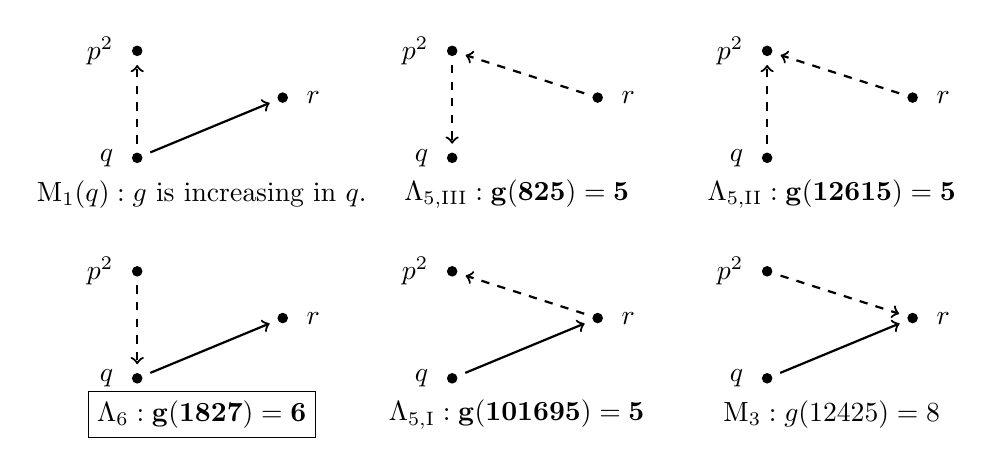
\begin{tikzpicture}
		%Figure 1
		\begin{scope}[shift={(0, 0)}]
			\node[point, label=left:$p^2$] (p1) {};
			\node[point, label=left:$q$, below=of p1] (q1) {};
			\node[point, label=right:$r$] at ($(q1) + (22.5:2)$)(r1) {};
			\node at ($(r1) + (230:1.6)$) {$\boxed{\Lambda_{6}: \mathbf{g(1827) = 6}}$};
		\end{scope}
		
		%Figure 2
		\begin{scope}[shift={(0, 2.8)}]
			\node[point, label=left:$p^2$] (p2) {};
			\node[point, label=left:$q$, below=of p2] (q2) {};
			\node[point, label=right:$r$] at ($(q2) + (22.5:2)$)(r2) {};
			\node at ($(r2) + (230:1.6)$) {$\m1(q) : g$ is increasing in $q$.};
		\end{scope}
		
		%Figure 3
		\begin{scope}[shift={(4, 0)}]
			\node[point, label=left:$p^2$] (p3) {};
			\node[point, label=left:$q$, below=of p3] (q3) {};
			\node[point, label=right:$r$] at ($(q3) + (22.5:2)$)(r3) {};
			\node at ($(r3) + (230:1.6)$) {$\qlame : \mathbf{g(101695) = 5}$};
		\end{scope}
		
		%Figure 4
		\begin{scope}[shift={(4, 2.8)}]
			\node[point, label=left:$p^2$] (p4) {};
			\node[point, label=left:$q$, below=of p4] (q4) {};
			\node[point, label=right:$r$] at ($(q4) + (22.5:2)$)(r4) {};
			\node at ($(r4) + (230:1.6)$) {$\qlamd : \mathbf{g(825) = 5}$};
		\end{scope}
		
		%Figure 5
		\begin{scope}[shift={(8, 0)}]
			\node[point, label=left:$p^2$] (p5) {};
			\node[point, label=left:$q$, below=of p5] (q5) {};
			\node[point, label=right:$r$] at ($(q5) + (22.5:2)$)(r5) {};
			\node at ($(r5) + (230:1.6)$) {$\m{3}: g(12425) = 8$};
		\end{scope}
		
		%Figure 6
		\begin{scope}[shift={(8, 2.8)}]
			\node[point, label=left:$p^2$] (p6) {};
			\node[point, label=left:$q$, below=of p6] (q6) {};
			\node[point, label=right:$r$] at ($(q6) + (22.5:2)$)(r6) {};
			\node at ($(r6) + (230:1.6)$) {$\qlamz: \mathbf{g(12615) = 5}$};
		\end{scope}
		
		\path[->, thick] (q2) edge[dashed] (p2) (q2) edge (r2)
		(q6) edge[dashed]  (p6) (r6) edge[dashed] (p6) (r4) edge[dashed] (p4);
		\path[->, thick] (q1) edge (r1) (q3) edge (r3) (q5) edge (r5);
		\path[->, thick] (r3) edge[dashed] (p3) (p5) edge[dashed] (r5);
		\path[->, thick] (p1) edge[dashed] (q1);
		\path[->, thick] (p4) edge[dashed] (q4);
	\end{tikzpicture}
\end{center}

\subsubsection*{Three edges in the \hg{1}}
We add one edge to an admissible graph with two edges which yields $g \le 6$, so one of $\qlame$, $\qlamz$, $\qlamd$ or $\Lambda_{6}$ from the previous section. It can be verified that the graphs arising from $\qlame$ and $\qlamz$ are regular.

In $\qlame$ the edge must be $q \dashrightarrow p^2$, otherwise we would get an acyclic grpah. In $\qlamz$, $q$ and $r$ are interchangeable, so assume we add $q \rightarrow r$. Finally, in $\Lambda_6$, we can add $p^2 \dashrightarrow r$, but this then we get $M_\text{II}$ as a proper subgraph, a contradiction. Representatives of the first two graphs are $35301 = 3\cdot7\cdot41^2$ for $\qlame$, $17661 = 3\cdot7\cdot29^2$, and GAP yields $g = 8, 13$, respectively. The final possibility is $\qlamd$. 
Adding $r \rightarrow q$ yields at least $2g(pqr) = 2 \cdot 2^2 = 8$ groups: Indeed, this is the number of groups of the form $\cyc{q} \rtimes (P \times \cyc{r})$. We conclude that there is no admissible graph with three edges.


\subsection{Admissible $n$ with $\lambda(n) = 5$ and $\mu(n) \ge 2$} 
There are three cases to consider.

\case{A} $n = p^3 q r$. We immediately see that $q$ and $r$ are not connected, as this would give 10 groups. We must have $g(p^3 q) = 6$. The case that yields the least number of groups is $r \mid p^3 - 1$ but not $r \mid p^2 - 1$, and in this case we get $2^2 = 4$ groups of the form $\cyc{p}^3 \rtimes \cyc{qr}$ and 4 groups of the form $P \times \cyc{qr}$, where $P$ is any group of order $p^3$ different from $\cyc{p}^3$. This gives a total of 8 groups, proving that $n$ is inadmissible.

\case{B} $n = p^2 q^2 r$. We must have $g(p^2 r) = g(p^2 r) = 3$, which means we have arrows $r \dashrightarrow p^2, q^2$. It is easy to see that there are $3^2 = 9$ groups of the form $(P \times Q) \rtimes \cyc{r}$, simply by observing that for each $P$ we can choose either $\cyc{p^2} or \cyc{p}^2$, and in the latter case, we can let $\cyc{r}$ act on it or not. Once again, $n$ is inadmissible.
 
\case{C} $n = p^2 q r s$.
If $qrs$ is cyclic, we get $g(p^2 q r) \le 6$ precisely if it is graph is $\qlamz$. An arrow $s \dashrightarrow p^2$ yields $2^3 = 8$ by a counting argument similar to the ones above, so we need $p^2 \rightarrow s$. We claim that we do have $g(n) = 7$ in this case, making use of the observation $g(p^2 q r) = g(p^2 q s) = 5$.

We first recall the structure of these five group of order $p^2 s r$: These are of the forms $(\cyc{s} \tilde{\rtimes} P) \times \cyc{r}$ and $(\cyc{s} \times P) \times \cyc{r}$, where the tilde denotes a nontrivial semidirect product. Finally, we have $(\cyc{p}^2 \tilde{\rtimes} \cyc{r}) \times \cyc{s}$. In the first two cases we can choose $P$ in two ways, so the total is $2 + 2 + 1 = 5$ groups, and it is easily seen that they are nonisomorphic. Thus these must be all of them. The crucial observation is that if $\cyc{p}^2$ is acted on by some $\cyc{\alpha}$, then it is centralized by $\cyc{s}$.

A group $G$ of order $n$ is solvable by Feit-Thompson's theorem {\cite{oddsolve}}, and by Hall's theorems {\cite[Theorem~3.13]{fgt}} we get subgroups $H_q$ and $H_r$ of orders $p^2 q r$ and $p^2 s r$, respectively. Observe first that a $q$-Sylow subgroup is cyclic, and $q$ is the smallest prime dividing $n$, so by, e.g., {\cite[Theorem~5.14]{fgt}}, we conclude that $H_r$ is normal, which means $G \cong H_r \rtimes \cyc{q}$. If $\cyc{q}$ acts nontrivially, then the $p$-Sylow subgorup of $G$ must be isomorphic to $\cyc{p}^2$, and by the observation in the previous paragraph, it must be centralized by $\cyc{s}$. There are precisely 2 such cases. If it acts trivially, we get 5 groups. This gives a total of 7 groups.

We move on to show that this is the only admissible case. Assume $qrs$ has one edge. We know that $n/v$ is connected for some prime $v \in {q, r, s}$, so assume it is $s$, and let $m = p^2 q r$. 

\case{C.1} \emph{There is an arrow $q \rightarrow r$.} By our work in section 3.3, the graph of $m$ is either $\qlame$ or $\Lambda_6$.

Assume it is $\qlame$. We can join $s$ to $p^2$ only, as $qrs$ has precisely one edge which is $q \rightarrow r$. Now an arrow $p^2 \dashrightarrow s$ means that the graph of $pqrs$ looks like a disjoint union of two \tikz[ww] \pic{walk};, so by \thref{eubold} we have $g(n) \ge 2 \cdot 4 = 8$. On the other hand, if we have an arrow $s \dashrightarrow p^2$, consider the groups of order $n$ with $\cyc{s}$ acting on $\cyc{p}^2$, either trivially or not. Now $\cyc{r}$ can act either trivially or not, and if it acts trivially, $\cyc{q}$ can act on it nontrivially. This gives 6 groups. On the other hand, we have 2 groups with a cyclic $p$-Sylow subgroup, depending on whether $\cyc{q}$ acts on $\cyc{r}$ or not. This gives a total of 8 groups, as claimed.

Now assume it is $\Lambda_6$. Once again, the arrow is either $s \dashrightarrow p^2$ or $p^2 \dashrightarrow s$. The latter case has $M_2$ as a proper subgraph, and $g(M_2) = 11$, so we only consider the first case. An argument similar to the last case shows that this also yields at least 8 groups.

\case{C.2} \emph{There is an edge linking to $s$.} By our work in section 3.3, the graph of $m$ is either $\qlamz$ or $\qlamd$.

Consider $\qlamd$. If $q$ is connected to $s$, then the graph of $pqs$ is connected, and thus we get at least 3 groups. By \thref{eubold}, this means we get at least 6 groups of order $p^2 qr$. There are two groups with $\cyc{p}^2$ as a direct factor, and we can let $\cyc{r}$ act nontrivialy on them to get two more new groups. This gives a total of 8 groups. We dismiss the other case, with $r$ connected to $s$, similarly: We have 3 groups with $\cyc{r}$ as a direct factor, and these give rise to 3 more groups with a nonabelian subgroup of order $rs$. This brings the total to $3 + 3 + 2 = 8$.

In $\qlamz$, $q$ and $r$ are indistinguishable, so we have two cases, $q \rightarrow s$ and $s \rightarrow q$. The first yields $\m1(q)$ as a proper subgraph, namely, that of $p^2 q s$, and consequently its $g$ is an increasing function that depends only on $q$. We already know that the minimum is 6 and is attained when $q = 3$. It can be seen that $163995 = 3 \cdot 5 \cdot 13 \cdot 29^2$ represents $p^2 q r s$ when $q = 3$, and $g(163995) = 10$ according to GAP. This shows that we cannot have $q \rightarrow s$. On the other hand, if we have $s \rightarrow q$, we recall that $g(\qlamz) = 5$. We have $g(p^2 r)g(qs) = 6$, so we have 6 groups with $qs$ as a direct factor. Now consider the groups $(\cyc{p}^2 \rtimes \cyc{q}) \times \cyc{rs}$ and $(\cyc{p}^2 \rtimes \cyc{qr}) \cyc{s}$, where the semidirect product is nontrivial (and $r$ acts nontrivially in the second group). These do not have a normal subgroup of order $qs$, and are therefore distinct from the 6 groups of earlier. This gives a total of 8 groups, showing that $n$ is indeed not admissible.

\emph{Conclusion.} Adding any more edges to the graph of $qrs$ can only increase $p^2 q r s$, so we have shown that $qrs$ must be cyclic, and thus the only admissible case is when the graph of $p^2 q r$ is $\qlamz$ and there is an arrow $p^2 \dashrightarrow s$.

\section{Summary of the results}
In what follows, $p, q, r, s$ represent distinct, odd primes.
\setenumerate[1]{label=\Roman*., font=\normalfont}
\begin{thm}
	For cyclic-free $n$, we have $g(n) = 6$ precisely when one of the following holds:
	\begin{enumerate} \listspace
		\item $n = pqrs$ where $r \equiv 1 \Mod{qs}$ and $q \equiv 1 \Mod{q}$,
		\item $n = 3p^2$ where $p \equiv 1 \Mod{3}$,
		\item $n = p^3 q$ where $p^3 \equiv 1 \Mod{q}$ but $p^2 \not\equiv 1 \Mod{q}$,
		\item $n = p^2 q r$ where $r \equiv 1 \Mod{q}$, and either $p \parallel q - 1$ or $q = 3$ and $p \equiv -1 \Mod{3}$,
		\item $n = p^2 q^2$ where $p \parallel q - 1$,
		\item $n = 2pq$ where $q \equiv 1 \Mod{p}$,
		\item $n = n_1 n_2$ where $n_1, n_2$ are arithmetically independent and
		\begin{enumerate}
			\item $n_1 = qr$ where $r \equiv 1 \Mod{q}$ or $n_1 = p^2$.
			\item $n_2 = pqr$ where $r \equiv 1 \Mod{q}$ and $q \equiv 1 \Mod{p}$ or $n_2 = p^2 q$ and $q \mid p + 1$.
		\end{enumerate}
	\end{enumerate} \textspace
	and in cases I-IV no further congruences of the form $\alpha \equiv \pm 1 \Mod{\beta}$ \nolinebreak[4] \mbox{occur}.
\end{thm}
\begin{thm}
	For cyclic-free $n$, we have $g(n) = 7$ precisely when one of the following holds:
	\begin{enumerate}	\listspace
		\item $n = 5pq$ where $p \equiv q \equiv 1 \Mod{5}$,
		\item $n = 3qr$ where $q \equiv r \equiv 1 \Mod{3}$ and $r \equiv 1 \Mod{q}$,
		\item $n = 3pqr$ where $p \equiv q \equiv 1 \Mod{3}$ and $r \equiv 1 \Mod{q}$,
		\item $n = 5p^2$ where $p \equiv 1 \Mod{5}$,
		\item $n = p^3 q$ where $p \equiv -1 \Mod{q}$,
		\item $n = 5p^2 q$ where $r \equiv 1 \Mod{5}$ and $p \equiv -1 \Mod{5}$,
		\item $n = p^2 q r s$ where $p \equiv -1 \Mod{qr}$ and $p \parallel s - 1$,
		\item $n = p^2 q^2$ where $p \parallel q + 1$,
	\end{enumerate} \textspace
	and in cases I-VII no further congruences of the form $\alpha \equiv \pm 1 \Mod{\beta}$ \nolinebreak[4] \mbox{occur}.
\end{thm}

\begin{center}\section*{References}\end{center}
\microtypesetup{protrusion=false}
\printbibliography[heading=none]

\end{document}